\documentclass[11pt,a4paper]{article}

% Codificacion, idioma y tipografia
\usepackage[utf8]{inputenc}
\usepackage[T1]{fontenc}
\usepackage[spanish, es-nodecimaldot]{babel}
\usepackage{lmodern}

% Pagina y elementos visuales
\usepackage[a4paper, margin=2.5cm]{geometry}
\usepackage{graphicx}
\usepackage{float}
\usepackage{booktabs}
\usepackage{array}
\usepackage{tabularx}
\usepackage{xcolor}
\usepackage{fancyhdr}
\usepackage{caption}
\usepackage{enumitem}
\usepackage{microtype}
\usepackage{amsmath}

% Codigo y enlaces
\usepackage{listings}
\usepackage[hidelinks]{hyperref}

\definecolor{codebg}{RGB}{245,247,250}
\definecolor{codecomment}{RGB}{70,110,70}
\definecolor{codekeyword}{RGB}{35,75,150}

\lstdefinelanguage{Cypher}{
	morekeywords={MATCH,OPTIONAL,WHERE,RETURN,WITH,ORDER,BY,ASC,DESC,LIMIT,
		CALL,YIELD,UNWIND,AS,AND,OR,NOT,IN,CASE,WHEN,THEN,END,DISTINCT},
	sensitive=false,
	morecomment=[l]{//},
	morestring=[b]'
}

\lstset{
	language=Cypher,
	inputencoding=utf8,
	extendedchars=true,
	basicstyle=\ttfamily\small,
	keywordstyle=\color{codekeyword}\bfseries,
	commentstyle=\color{codecomment},
	backgroundcolor=\color{codebg},
	frame=single,
	rulecolor=\color{black!20},
	breaklines=true,
	keepspaces=true,
	columns=fullflexible,
	showstringspaces=false,
	upquote=true,
	numbers=left,
	numberstyle=\tiny\color{black!50},
	xleftmargin=1.5em,
	framexleftmargin=1.2em,
	literate={á}{{\'a}}1 {é}{{\'e}}1 {í}{{\'i}}1 {ó}{{\'o}}1 {ú}{{\'u}}1
	          {Á}{{\'A}}1 {É}{{\'E}}1 {Í}{{\'I}}1 {Ó}{{\'O}}1 {Ú}{{\'U}}1
	          {ñ}{{\~n}}1 {Ñ}{{\~N}}1 {ü}{{\"u}}1 {Ü}{{\"U}}1
	          {¿}{{?`}}1 {¡}{{!`}}1
}

\setlist{nosep}
\setlength{\parindent}{0pt}
\setlength{\parskip}{0.6em}

\pagestyle{fancy}
\fancyhf{}
\lhead{Bases de Datos Avanzadas}
\rhead{Tarea 3: Neo4j}
\cfoot{\thepage}
\setlength{\headheight}{14pt}

% Inserta una captura: archivo, ancho relativo, pie de figura y etiqueta
\newcommand{\captura}[4]{%
	\begin{figure}[H]
		\centering
		\includegraphics[width=#2\textwidth]{img/#1}
		\caption{#3}
		\label{#4}
	\end{figure}}

\begin{document}

\begin{titlepage}
	\centering
	\vspace*{1cm}
	{\Large Universidad Técnica Federico Santa María\\}
	{\large Campus Santiago San Joaquín\\[0.3em]
	Bases de Datos Avanzadas\\[3cm]}
	{\Huge\bfseries Tarea 3: Neo4j\\[1.5cm]}
	{\Large Informe\par}
	\vfill
	\begin{tabular}{rl}
		\textbf{Nombre:} & Sebastián Andrés Santander Martínez\\
		\textbf{Rol:} & 202373608-2\\[0.5em]
		\textbf{Nombre:} & Jaime Guzmán Muñoz\\
		\textbf{Rol:} & 202373524-8\\
	\end{tabular}
	\vfill
	Segundo semestre 2026
\end{titlepage}

\tableofcontents
\newpage

\section{Introducción}

En esta tarea se trabaja con Neo4j, una base de datos NoSQL orientada a grafos. A diferencia
de MongoDB y Cassandra, que usamos en las tareas anteriores, acá la información se guarda como
nodos y relaciones con propiedades, y las consultas se escriben en Cypher describiendo patrones
de conexión entre ellos.

El caso es el de la noche de Halloween. 15 estudiantes de INF325 salieron a pedir dulces a las
10 casas cercanas a la universidad, cada uno visitó 5 casas distintas y anotó cuántos dulces
recibió en cada una. Se dejó ese registro como grafo en el archivo \texttt{tarea.dump}
y el objetivo es encontrar al ganador y analizar cómo se conectan estudiantes y casas, sin
generar ni modificar datos. Primero se exploró el grafo con consultas Cypher, después se
aplicaron los algoritmos Degree Centrality y Node Similarity de la biblioteca Graph Data
Science (GDS) y por último se buscaron caminos entre estudiantes.

Todas las consultas están en el archivo \texttt{consultas.cypher}, en el mismo orden de este
informe. Ese archivo y las capturas también están en el repositorio público
\url{https://github.com/Sxbayb/Tareas-BDDA}.

\section{Preparación del entorno}

\subsection{Instalación de Neo4j y carga de datos}

Se usó Neo4j Desktop con una instancia local llamada \texttt{tarea3} en la versión 2026.10.1 de
Neo4j. La instancia se creó directamente desde el respaldo, seleccionando \texttt{tarea.dump} en
la opción de carga de la ventana \textit{Create Instance}. Desktop carga ese archivo en la base
\texttt{neo4j}, que es la base sobre la que se ejecutaron todas las consultas del informe.

\begin{figure}[H]
	\centering
	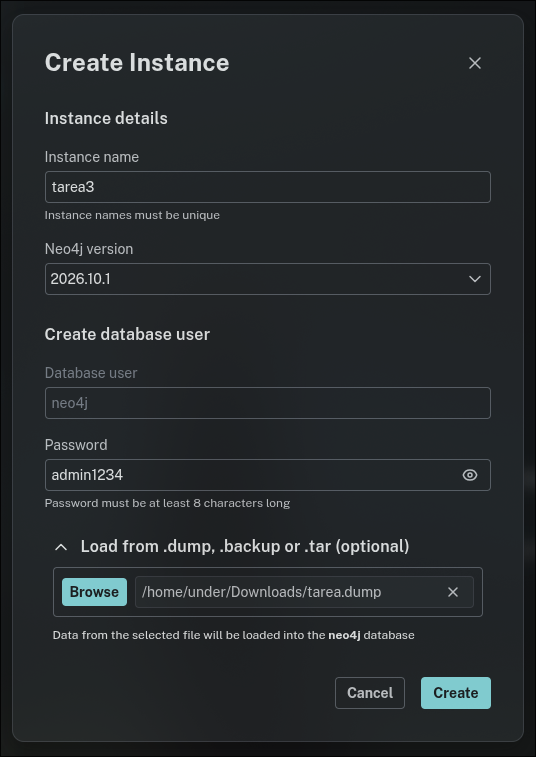
\includegraphics[width=0.7\textwidth]{img/creacionInstancia.png}
	\caption{Creación de la instancia y carga de archivo dump.}
	\label{fig:instancia}
\end{figure}

\subsection{Instalación y verificación GDS}

El plugin Graph Data Science se instaló desde la sección \textit{Plugins} de la instancia. La
consulta \texttt{RETURN gds.version()} devuelve la versión 2026.10.1, lo que confirma que la
biblioteca quedó disponible en la instancia.

\begin{figure}[H]
	\centering
	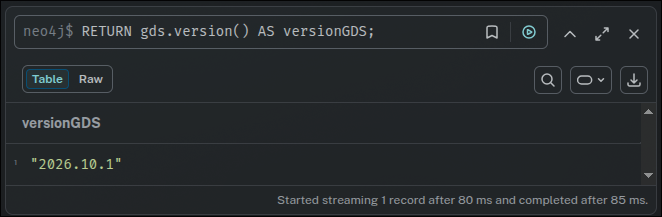
\includegraphics[width=0.7\textwidth]{img/gdsVersion.png}
	\caption{Descarga y comprobación de versión de GDS.}
	\label{fig:gds}
\end{figure}

\subsection{Verificación de carga}

Las tres consultas de verificación devuelven 15 estudiantes, 10 casas y 75 visitas, que son los
valores esperados, así que la carga del respaldo quedó completa.

\begin{figure}[H]
	\centering
	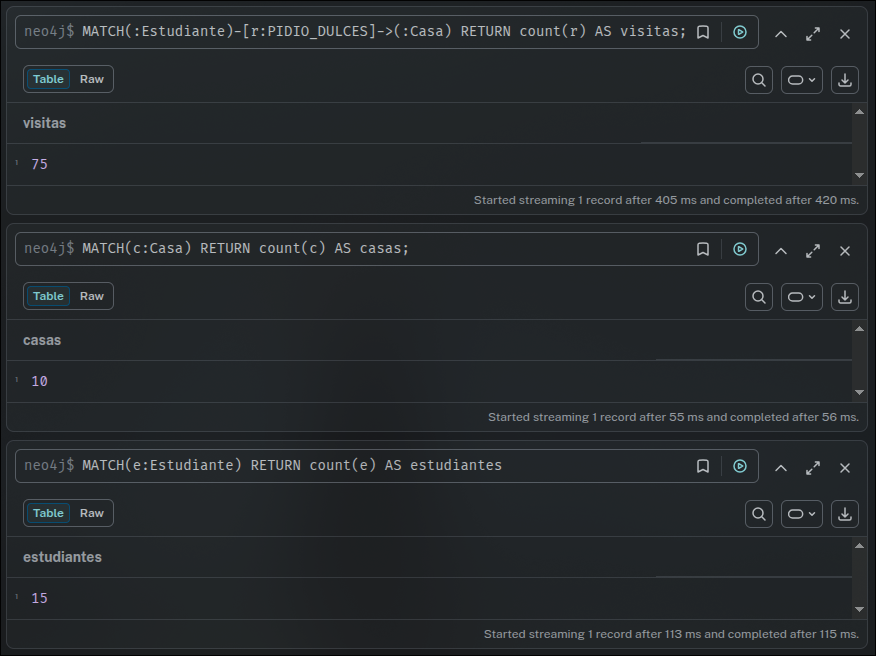
\includegraphics[width=0.7\textwidth]{img/consultasVerificacion.png}
	\caption{Conteo de estudiantes, casas y visitas.}
	\label{fig:verificacion}
\end{figure}

\section{Parte 1: Exploración y consultas Cypher}
\subsection{Visualización e interpretación del grafo}
\begin{figure}[H]
	\centering
	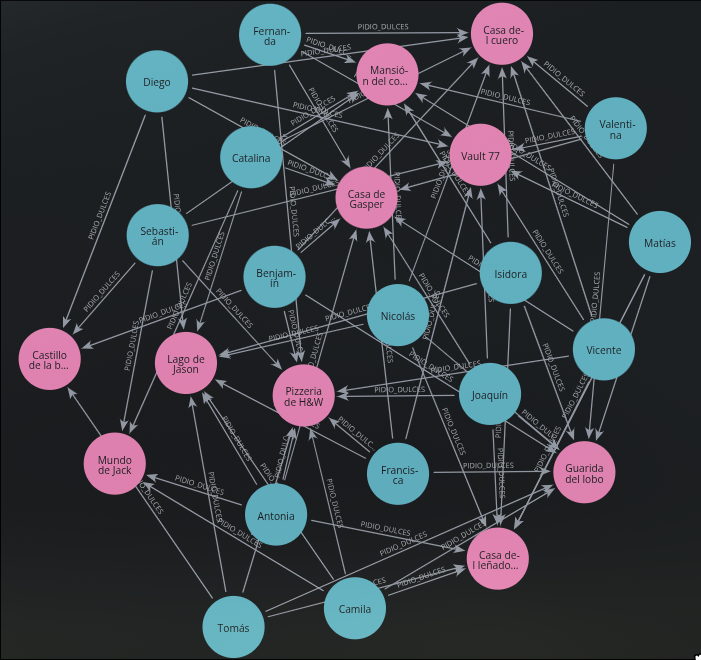
\includegraphics[width=0.7\textwidth]{img/test.png}
	\caption{Grafo completo, con estudiantes en azul y casas en rosado.}
	\label{fig:grafo}
\end{figure}
En el grafo presentado se pueden observar dos tipos de nodos. El primer tipo de nodo que se puede ver son los 
\textbf{nodos de estudiantes}(nodos azules) los cuales representan a cada uno de los 15 estudiantes del curso
que salieron a pedir dulces. Su propiedad principal es \texttt{id}, la cual almacena como \texttt{strings} el
nombre del estudiante. El otro tipo de nodo que se puede ver son los \textbf{nodos de las casas}(nodos rosados)
los cuales representan cada una de las 10 casas disponibles para pedir dulces. Posee una propiedad \texttt{id}
numérica y una propiedad \texttt{direccion} que contiene su nombre temático.


Se puede apreciar en el grafo como se tienen relaciones dirigidas, el sentido que se puede apreciar es que la dirección 
va siempre desde un \textbf{nodo estudiante} a un \textbf{nodo casa}. Cada relación refleja la acción física y semántica
de la actividad: es el estudiante quien actúa como emisor u origen de la visita, desplazándose hacia la casa como lugar 
de destino. Una arista representa el hecho de que ese estudiante visitó esa casa específica, independientemente de si
recibió o no dulces.

Cada relación \texttt{PIDIO\_DULCES} almacena dos propiedades:
\begin{itemize}
	\item \texttt{cantidad}: Representa el número de dulces obtenidos en esa visita puntual. Puede ser 0 (no recibe dulces), 1 (recibió un dulce) o 2 (recibió dos dulces).
	\item \texttt{tipo}: Registra la variedad del dulce recibido, toma valor \texttt{'Ninguno'} en caso de que la \texttt{cantidad} sea 0.
\end{itemize}

Como ejemplo, la visita de Antonia a Mundo de Jack (que aparece en la Figura \ref{fig:visitas0}) es una relación
que sale del nodo de Antonia y llega a la casa Mundo de Jack, con \texttt{cantidad = 0} y \texttt{tipo = 'Ninguno'}.
Es decir, Antonia fue a esa casa pero no le dieron dulces, y aun así la visita queda registrada en el grafo.

En la visualización aparecen los 15 estudiantes y las 10 casas, lo que coincide con los conteos de la verificación
de carga. Como ninguna casa quedó sin visitas, no hay nodos aislados que se pierdan al mostrar solo las relaciones.

En teoría de grafos, un grafo es bipartito si un conjunto de vértices $V$ puede dividirse en dos subconjuntos 
disjuntos e independientes, tales que toda arista de $E$ conecta un vértice de $V_1$ con uno de $V_2$. En este modelo
es posible apreciar como tenemos todos los nodos particionados en dos clases independientes: $V_1=\text{Estudiantes}$ y
$V_2=\text{Casas}$. Además, todas las relaciones van exclusivamente entre un elemento de $V_1$ y un elemento de $V_2$. 
Por último, no hay ninguna relación que conecte a un estudiante con otro estudiante, ni existe ninguna relación que conecte
una casa con otra casa.

Por estas razones es posible decir que el grafo con el que se está trabajando es un grafo bipartito.

\subsection{Casa con más visitas}
\begin{figure}[H]
	\centering
	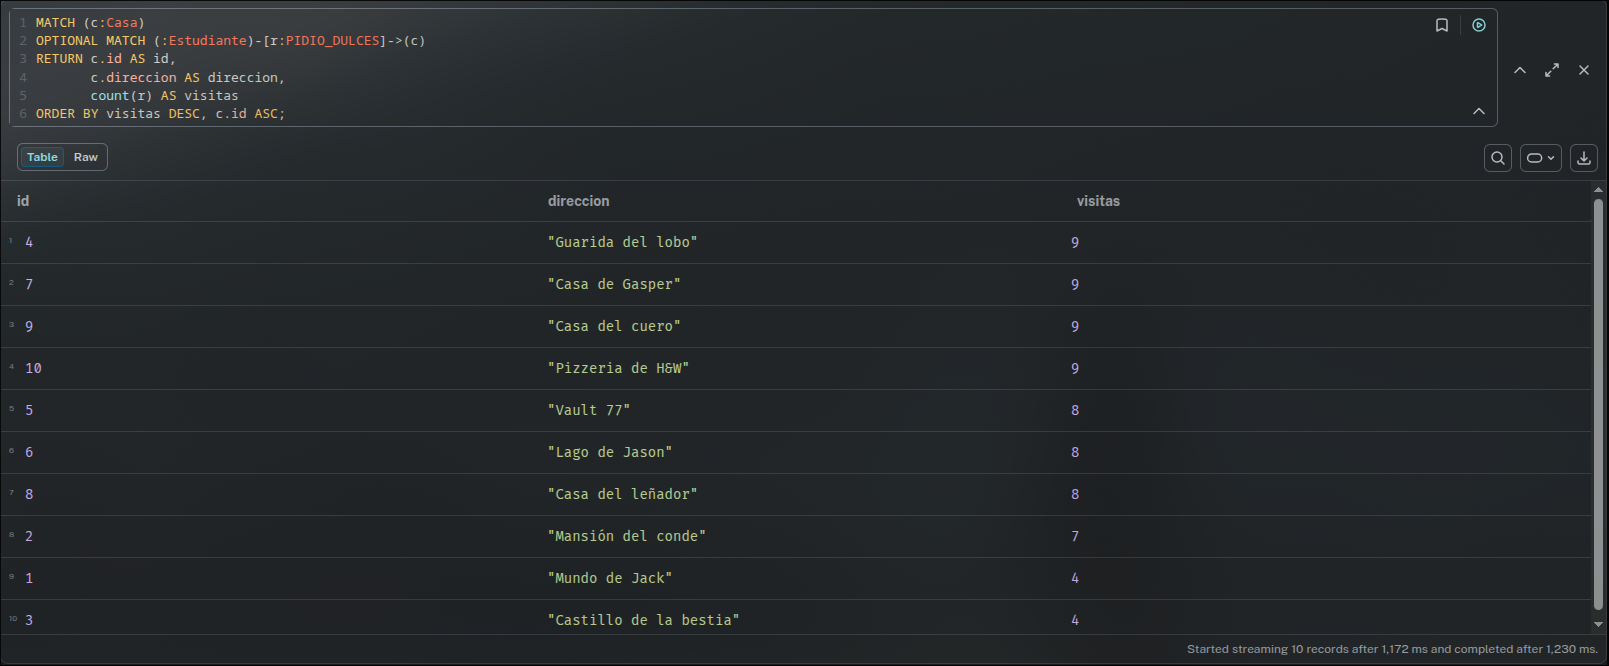
\includegraphics[width=1\textwidth]{img/ranking10casas.png}
	\caption{Ranking de las 10 casas con más visitas.}
	\label{fig:rankingCasas}
\end{figure}

\begin{figure}[H]
	\centering
	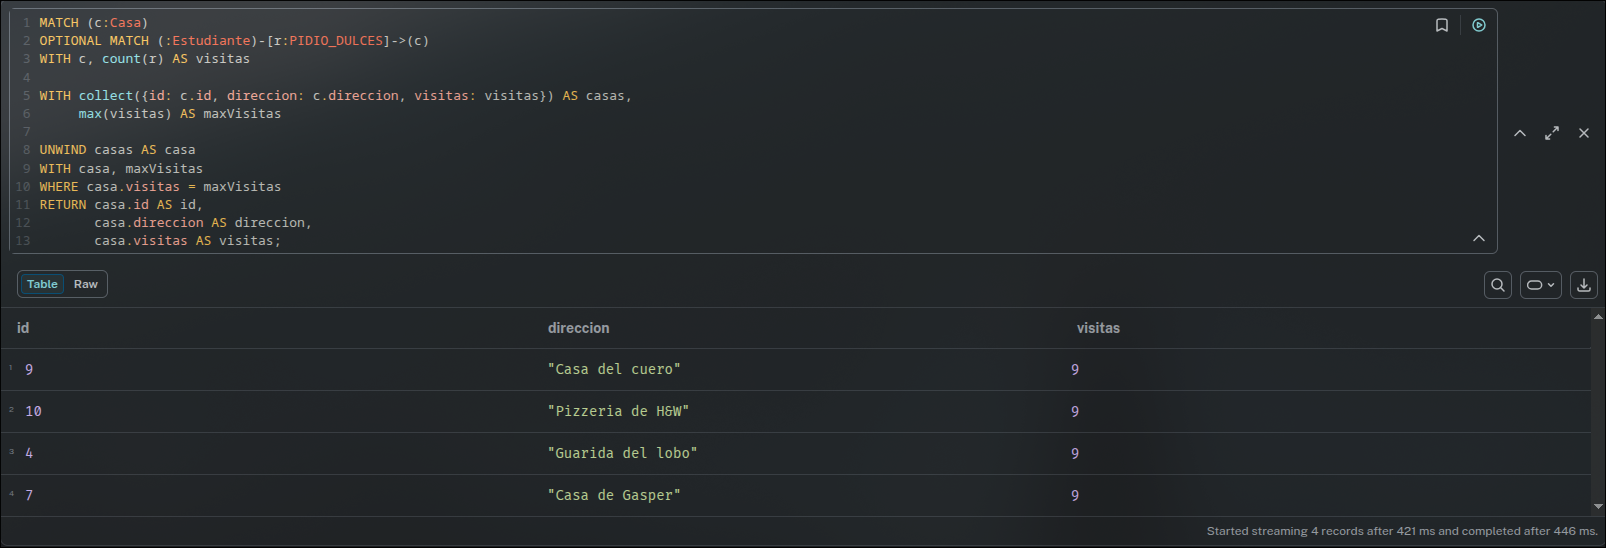
\includegraphics[width=1\textwidth]{img/empateCasas.png}
	\caption{Empate en casas con más visitas.}
	\label{fig:empateCasas}
\end{figure}

El ranking muestra que no hay una sola casa ganadora. Cuatro casas comparten el máximo de 9 visitas: Guarida del lobo (id 4),
Casa de Gasper (id 7), Casa del cuero (id 9) y Pizzeria de H\&W (id 10). Les siguen Vault 77, Lago de Jason y Casa del leñador
con 8 visitas, Mansión del conde con 7, y al final Mundo de Jack y Castillo de la bestia con 4. Ninguna casa quedó con cero
visitas, y la suma del ranking da exactamente las 75 visitas del grafo.

Para este contexto se debe considerar una visita que tenga \texttt{cantidad=0} ya que la existencia de la relación dirigida
representa el hecho de que un estudiante se trasladó y visitó esa casa puntual durante Halloween. La relación existe independiente
del resultado de la interacción. El hecho de que la propiedad \texttt{cantidad} tome un valor de 0 modela una visita infructuosa
(por ejemplo, nadie atendió la puerta o ya no había dulces), pero la casa efectivamente fue visitada por el estudiante. Como se
pide medir la afluencia de visitas recibidas por la casa, sería un error descartar la arista o solo sumar los dulces entregados
por una casa, ya que eso mediría el inventario de dulces entregados y no el tráfico de personas que acudieron al lugar.

\subsection{Estudiante con más dulces}
\begin{figure}[H]
	\centering
	\vbox{\offinterlineskip
		\hbox{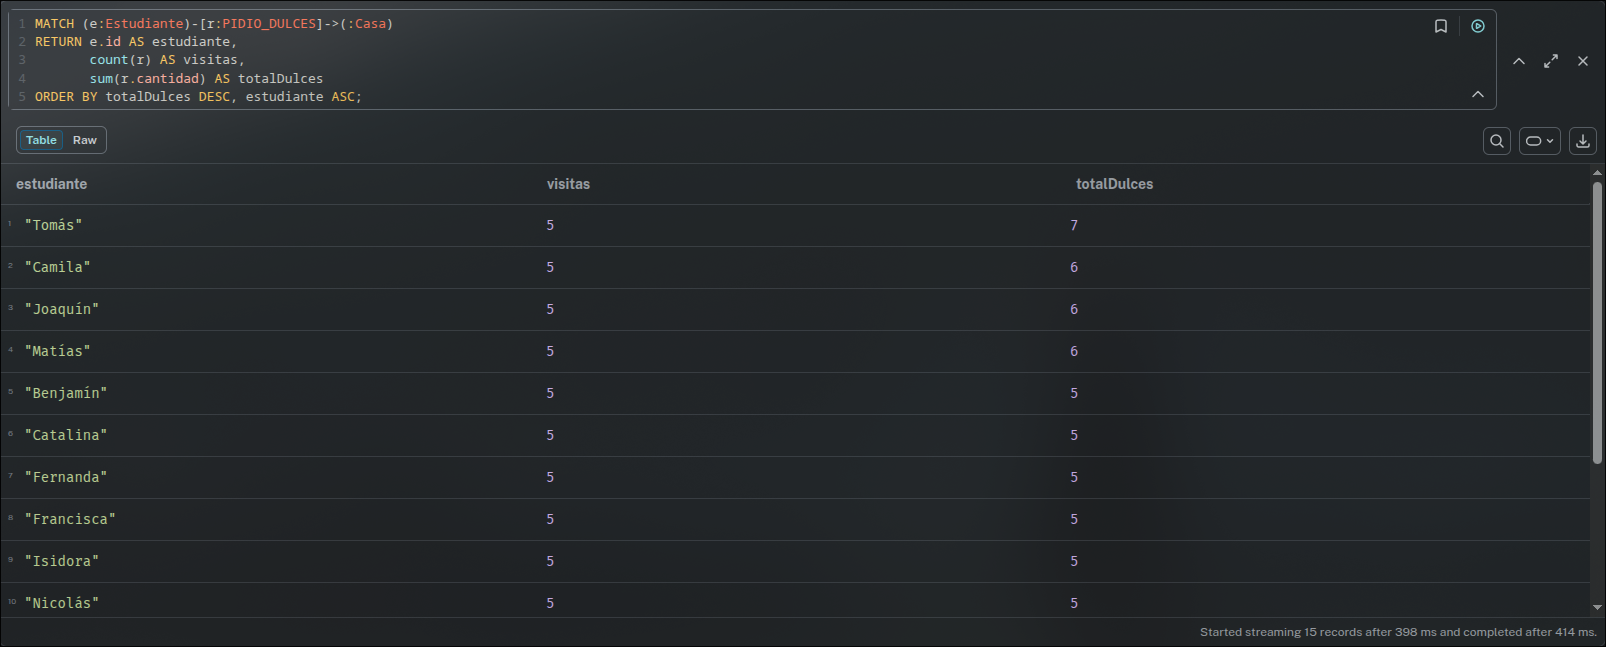
\includegraphics[width=1\textwidth]{img/ranking10estudiantes.png}}
		\hbox{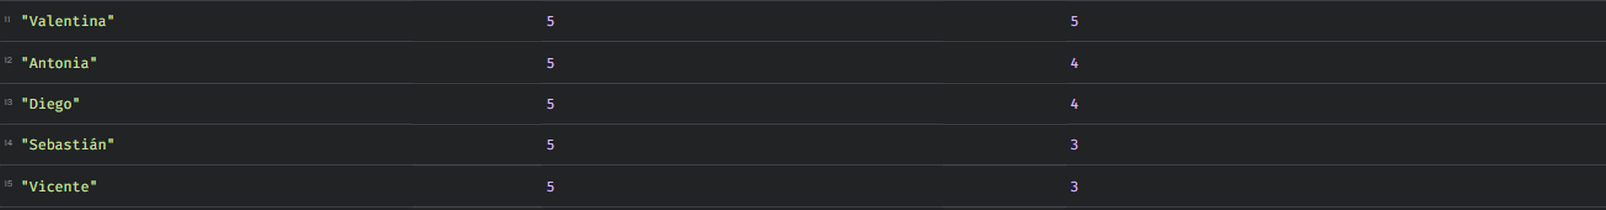
\includegraphics[width=1\textwidth]{img/ranking10estudiantes2.png}}}
	\caption{Ranking de los 15 estudiantes según dulces obtenidos.}
	\label{fig:rankingEstudiantes}
\end{figure}

\begin{figure}[H]
	\centering
	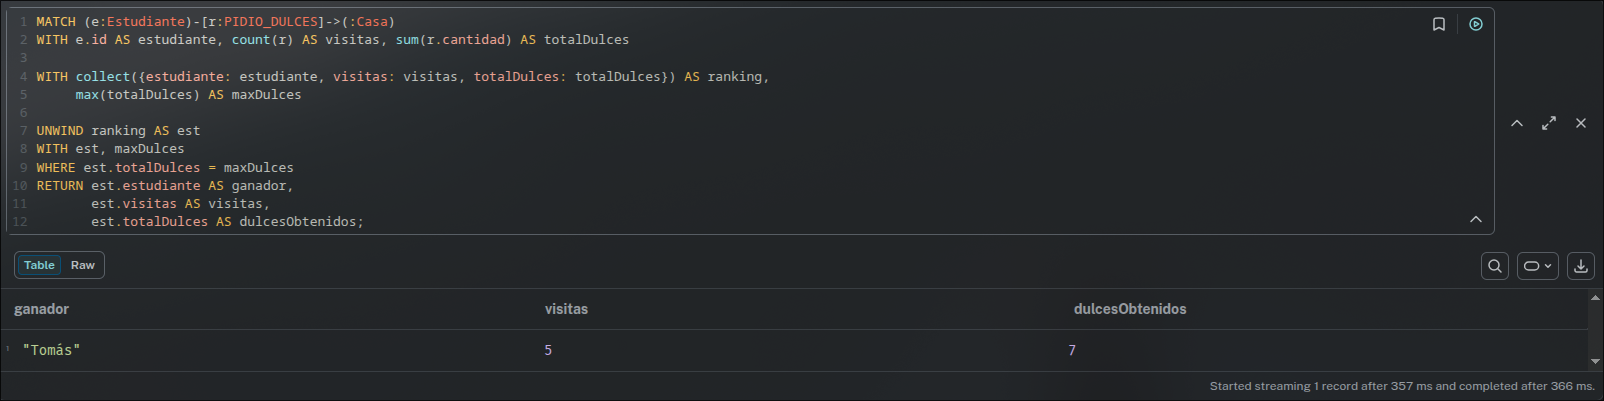
\includegraphics[width=1\textwidth]{img/empateEstudiantes.png}
	\caption{Estudiante con más dulces.}
	\label{fig:empateEstudiantes}
\end{figure}

El ganador del bonus es Tomás, que es el único estudiante que alcanza el máximo con 7 dulces en sus 5 visitas, por lo que no hay
empate en el primer lugar. Más atrás quedan Camila, Joaquín y Matías, que empatan con 6 dulces, y los que menos obtuvieron
fueron Sebastián y Vicente, con 3.

Contar las visitas es una métrica estructural que mide el grado de salida del estudiante en el grafo, reflejando únicamente la 
cantidad de aristas o conexiones que posee. En cambio, sumar dulces cuantifica el valor acumulado de una propiedad numérica
propia de cada relación. Dado que cada visita puede otorgar 0, 1 y 2 dulces, contar aristas solo indica el número de lugares 
concurridos, mas no el beneficio o recompensa total obtenida.

El modelo fija como regla que cada estudiante visita exactamente 5 casas distintas, por lo que el conteo estructural de visitas
es idéntico para todos. No obstante, el resultado de cada visita es independiente y asigna valores de 0, 1 y 2 dulces de forma
estocástica. Debido a esta variabilidad en la propiedad \texttt{cantidad}, la suma total de cada alumno puede variar dentro del
rango de 0 a 10 dulces, produciendo totales finales distintos a pesar de tener la misma cantidad de visitas.

\subsection{Visitas sin dulces}
\begin{figure}[H]
	\centering
	\vbox{\offinterlineskip
		\hbox{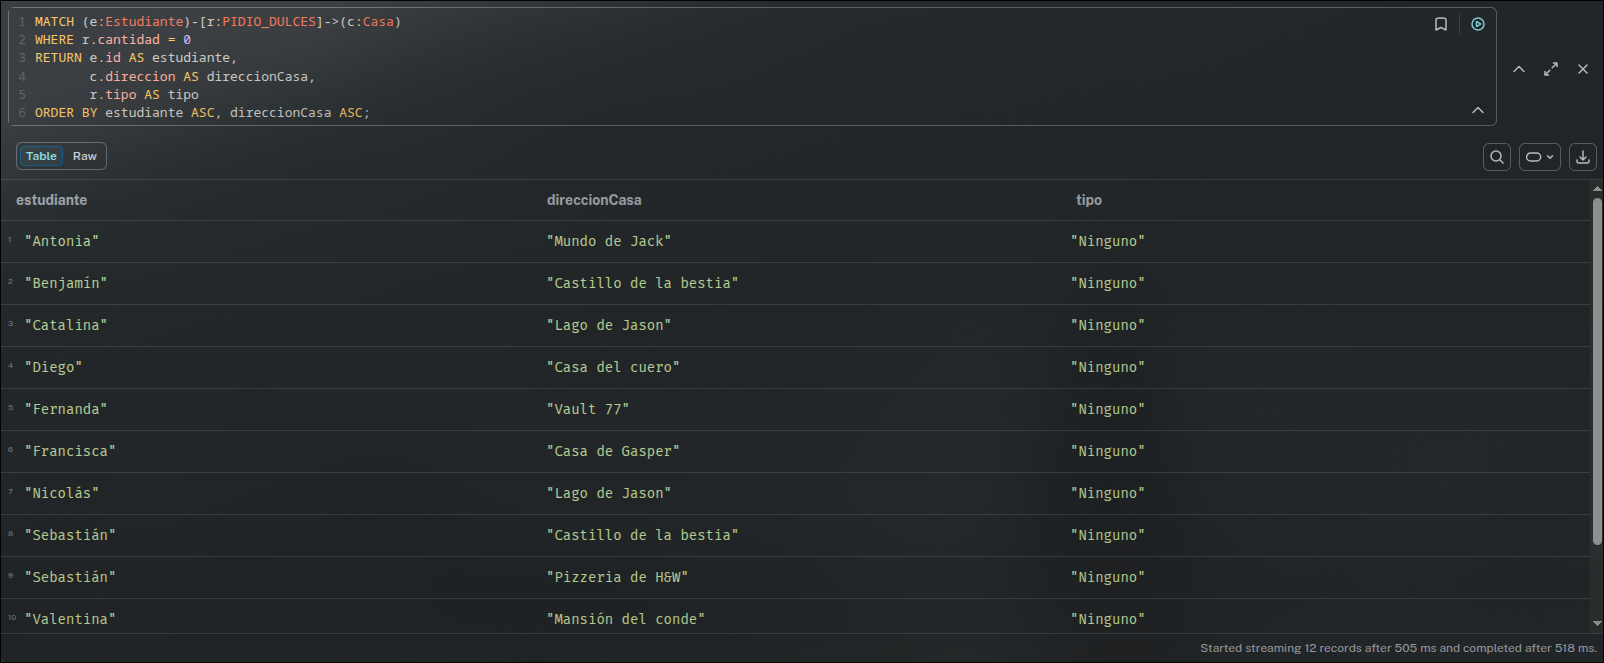
\includegraphics[width=1\textwidth]{img/visitasCantidad0.png}}
		\hbox{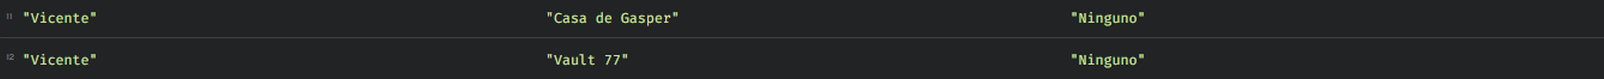
\includegraphics[width=1\textwidth]{img/visitasCantidad0_2.png}}}
	\caption{Visitas sin dulces.}
	\label{fig:visitas0}
\end{figure}

\begin{figure}[H]
	\centering
	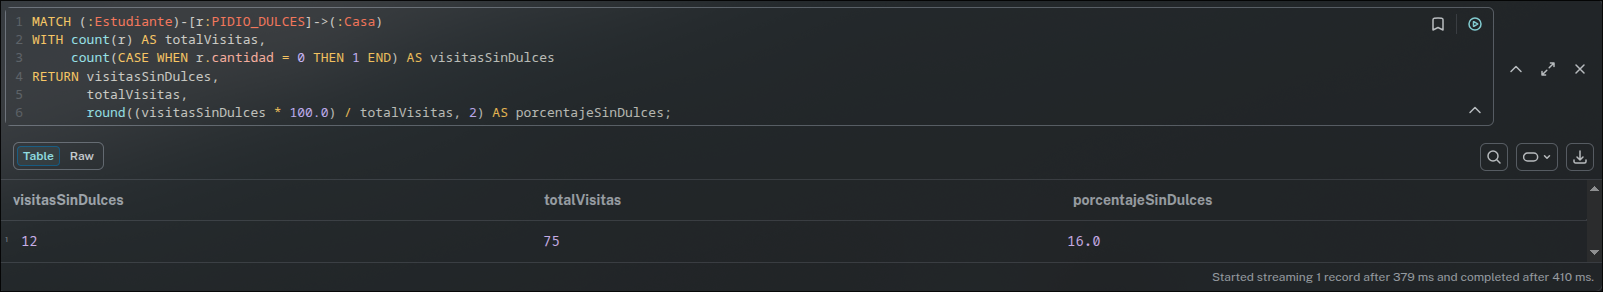
\includegraphics[width=1\textwidth]{img/porcentajeSinDulces.png}
	\caption{Porcentaje de visitas sin dulces.}
	\label{fig:porcentaje0}
\end{figure}

La consulta encuentra 12 visitas con \texttt{cantidad = 0}, todas con tipo \texttt{'Ninguno'}, lo que corresponde a
$12/75 = 0{,}16$, es decir, un 16\% de las 75 visitas. El porcentaje se calcula multiplicando por \texttt{100.0} para que
Cypher use aritmética decimal y no división entera.

Durante la generación de la base de datos, la asignación de dulces en cada visita se modeló como un experimento estocástico 
independiente con una probabilidad teórica del 20\% para el resultado \texttt{cantidad=0}. La discrepancia entre el porcentaje
real observado en la consulta (16\%) y dicho 20\% se fundamenta en principios estadísticos y en el tamaño de la muestra:
\begin{itemize}
	\item \textbf{Muestra finita y variabilidad muestral:} La base registra un universo total de exactamente 75 visitas. Según la ley de los grandes números, la frecuencia relativa observada de un evento converge a su probabilidad teórica únicamente cuando el número de repeticiones tiende a infinito. En un conjunto acotado de 75 eventos, el 20\% representa una esperanza matemática de $75\times0.20=15$ visitas teóricas, mas no una cota determinista o forzada.
	\item \textbf{Independencia de los eventos generados:} Cada visita fue asignada de forma pseudoaleatoria e independiente. El algoritmo no aplicó cuotas rígidas para asegurar que exactamente 15 de las 75 relaciones tuvieran valor cero, por lo que cualquier fluctuación observada en torno a la media esperada constituye una desviación muestral natural y propia de un proceso probabilístico discreto.
\end{itemize}

\section{Parte 2: Análisis con GDS}

\subsection{Proyección del grafo}

\captura{proyeccion.png}{0.8}{Creación de la proyección \texttt{halloween}.}{fig:proyeccion}

Proyectar el grafo significa cargar una copia de su estructura en el catálogo de GDS, que es
la memoria donde se ejecutan los algoritmos. La proyección no crea una segunda base de datos ni
modifica los nodos y relaciones guardados, así que se puede crear y eliminar sin afectar los
datos del caso. La consulta devuelve la proyección \texttt{halloween} con 25 nodos, que son los
15 estudiantes más las 10 casas, y 75 relaciones, lo mismo que se obtuvo en la verificación de
carga.

La orientación \texttt{NATURAL} indica que las relaciones se proyectan con la misma dirección
que tienen en la base, es decir, desde cada estudiante hacia la casa que visitó. No hace falta
proyectar la propiedad \texttt{cantidad} porque los análisis pedidos son sin pesos. Degree
Centrality solo cuenta relaciones y Node Similarity solo revisa qué casas son vecinas de cada
estudiante, así que el número de dulces no participa en ninguno de los dos cálculos.

\subsection{Degree Centrality: centralidad de las casas}

\captura{degreeRanking.png}{1}{Ranking de las 10 casas según Degree Centrality.}{fig:degreeRanking}

Con la orientación \texttt{NATURAL} el grado de un nodo cuenta sus relaciones de salida. Como
todas las relaciones van de estudiante a casa, cada estudiante tendría grado 5 y cada casa grado
0, lo que no sirve para medir las visitas recibidas. Con \texttt{REVERSE} el algoritmo recorre
las relaciones en sentido contrario dentro de la proyección, sin cambiarlas en la base, y el
puntaje de cada casa pasa a ser su grado de entrada, o sea, el número de estudiantes que llegaron
a ella. El filtro \texttt{WHERE nodo:Casa} se aplica después de ejecutar el algoritmo. De esta
forma la proyección conserva los dos tipos de nodos con todas sus conexiones y los estudiantes
solo se ocultan en el resultado final.

Para identificar todos los empates en el máximo se usó la misma idea de la Parte 1, calculando el
puntaje máximo y quedándose con las casas que lo alcanzan.

\captura{degreeMaximos.png}{1}{Casas empatadas en el puntaje máximo de Degree Centrality.}{fig:degreeMaximos}

Las casas con mayor centralidad son Guarida del lobo, Casa de Gasper, Casa del cuero y Pizzeria
de H\&W, empatadas con puntaje 9. Para compararlas con la Parte 1 se juntó en una sola consulta el
puntaje de GDS, el conteo de visitas hecho con Cypher y la suma de dulces que entregó cada casa.

\captura{degreeComparacion.png}{1}{Grado de entrada, visitas contadas con Cypher y dulces entregados por casa.}{fig:degreeComparacion}

Los puntajes coinciden con las visitas de la Parte 1 en las 10 casas: 9 para las cuatro casas
del máximo, 8 para Vault 77, Lago de Jason y Casa del leñador, 7 para Mansión del conde y 4 para
Mundo de Jack y Castillo de la bestia. Es lo esperable, porque en un grafo sin pesos el grado de
entrada de una casa es justamente la cantidad de relaciones \texttt{PIDIO\_DULCES} que llegan a
ella, que es lo mismo que cuenta \texttt{count(r)} en Cypher. La única diferencia es que GDS
entrega el puntaje como número decimal.

En este caso, tener mayor centralidad significa que la casa recibió más visitas, o sea que fue la
más elegida por los estudiantes y la que tiene más conexiones en el grafo. Eso no garantiza que
haya entregado más dulces, porque cada visita suma 1 al grado sin importar su cantidad, y una
visita con 0 dulces pesa lo mismo que una con 2. Por ejemplo, Pizzeria de H\&W es una de las casas
con grado 9, pero Sebastián no recibió dulces ahí. La tabla de comparación lo muestra con números.
Casa de Gasper y Pizzeria de H\&W tienen grado 9 y entregaron 8 dulces cada una, mientras que Casa
del leñador, con grado 8, entregó 9. Incluso entre las cuatro casas del máximo hay diferencias
grandes, ya que Guarida del lobo entregó 13 dulces con las mismas 9 visitas. La suma de la columna
\texttt{dulcesEntregados} da 74, igual que la suma de los totales de los 15 estudiantes en la
Parte 1, porque son los mismos dulces contados desde las casas en vez de desde los estudiantes.

\subsection{Node Similarity: estudiantes con visitas parecidas}

Node Similarity compara cada par de estudiantes según sus vecinos de salida, que en esta
proyección son las casas que visitó cada uno. Las casas no tienen relaciones de salida, por lo que
no se comparan entre sí. Con \texttt{topK: 14} cada estudiante puede quedar comparado con los
otros 14, y el umbral \texttt{similarityCutoff: 0.0001} deja fuera las parejas que no comparten
ninguna casa. Como el algoritmo devuelve cada pareja dos veces, una como (A, B) y otra como (B, A),
se filtró con \texttt{estudiante1 < estudiante2} para que aparezca una sola vez. En caso de empate
en el quinto lugar se ordenó también por nombre, para mostrar exactamente cinco parejas.

\captura{similitudTop5.png}{1}{Las 5 parejas de estudiantes con mayor similitud de Jaccard.}{fig:similitudTop5}

La pareja con mayor similitud es Isidora y Nicolás, con puntaje 1.0, y es la única con ese valor.
Las otras cuatro parejas del top son Antonia y Camila, Camila y Tomás, Fernanda y Valentina, y
Fernanda y Vicente, todas con 0,667, que corresponde a compartir 4 casas sobre 6 casas distintas en total. Como
esas cuatro empatan, el orden entre ellas lo define el desempate por nombre, y si hubiera más
parejas con 0,667 quedarían fuera del top solo por ese orden. Para el resto del análisis se eligió
la primera pareja, Isidora y Nicolás. Después se listaron las casas de cada uno y las casas
que visitaron ambos.

\captura{casasPorEstudiante.png}{1}{Casas visitadas por cada estudiante de la pareja.}{fig:casasPorEstudiante}

\captura{casasCompartidas.png}{1}{Casas que visitaron ambos estudiantes.}{fig:casasCompartidas}

La similitud de Jaccard divide las casas que los dos tienen en común por el total de casas
distintas que visitaron entre ambos. Isidora y Nicolás visitaron las mismas 5 casas (Mansión del
conde, Guarida del lobo, Lago de Jason, Casa del leñador y Casa del cuero), así que tienen 5 casas
en común sobre 5 casas distintas en total, lo que da $5/5 = 1$, el mismo valor que entregó GDS.
Para comprobarlo también se hizo el cálculo con Cypher.

\captura{jaccardCypher.png}{1}{Cálculo de la similitud de Jaccard con Cypher.}{fig:jaccardCypher}

La consulta devuelve 5 visitas para cada uno, una intersección de 5 casas, una unión de 5 y un
valor de Jaccard de 1.0, igual que el cálculo manual y que GDS.

Un resultado cercano a 1 significa que los dos estudiantes visitaron casi las mismas casas, y un 1
exacto, como el de esta pareja, significa que fueron a las mismas 5. Eso no implica que hayan obtenido la misma cantidad ni el
mismo tipo de dulces. La proyección no incluye \texttt{cantidad} ni \texttt{tipo}, así que el
algoritmo solo ve si existe la relación entre el estudiante y la casa. Además, en una misma casa
cada visita tiene su propio resultado. En la Figura \ref{fig:patronTabla} se ve lo que recibió cada
uno en las casas que comparten. En Guarida del lobo Isidora recibió 1 dulce y Nicolás 2, y en Lago
de Jason Isidora recibió un Chocolate (MVP) mientras que Nicolás se fue sin nada. Los tipos también
cambian, por ejemplo en Casa del leñador a Isidora le tocó un Masticable de platano y a Nicolás un
Chocolate (MVP). Los dos terminan con 5 dulces, pero repartidos de otra forma y de tipos
distintos, así que una similitud de 1 solo dice que fueron a los mismos lugares.

\section{Parte 3: Búsqueda de caminos}

\subsection{Casas compartidas}

Se usó la misma pareja de Node Similarity, Isidora y Nicolás. La primera consulta devuelve el
patrón completo para la vista de grafo y la segunda muestra lo mismo en tabla, junto con lo que
recibió cada uno en esas casas.

\captura{patronCompartido.png}{0.7}{Patrón entre los dos estudiantes y sus casas compartidas.}{fig:patronCompartido}

\captura{patronTabla.png}{1}{Casas compartidas y lo que recibió cada estudiante en ellas.}{fig:patronTabla}

Los dos estudiantes comparten sus 5 casas: Mansión del conde, Guarida del lobo, Lago de Jason,
Casa del leñador y Casa del cuero. Por eso la vista de grafo muestra 7 nodos, que son los 2
estudiantes y las 5 casas, y 10 relaciones, 5 de cada estudiante. Cada casa compartida forma un
camino de longitud 2 entre ellos, porque se pasa por dos relaciones. La primera sale de Isidora y
llega a la casa, y la segunda sale de Nicolás y llega a esa misma casa. Como no hay relaciones
directas entre estudiantes, la casa en común es lo único que los conecta, y cada una de las 5
casas compartidas aporta un camino distinto de largo 2.

\subsection{Camino más corto}

\captura{caminoCortoTabla.png}{1}{Camino más corto entre la pareja, con su longitud y recorrido.}{fig:caminoCortoTabla}

\captura{caminoCortoGrafo.png}{0.5}{Vista de grafo del camino más corto.}{fig:caminoCortoGrafo}

El camino encontrado tiene longitud 2 y recorre Isidora, Casa del leñador y Nicolás. En la
columna \texttt{recorrido} se muestra la dirección de las casas y el nombre de los estudiantes,
para que el camino se pueda leer sin revisar los identificadores internos. No puede existir un
camino de largo 1 porque eso sería una relación directa entre dos estudiantes, y como la pareja
comparte al menos una casa ya existe uno de largo 2. Como esta pareja comparte 5 casas, existen 5 caminos
mínimos distintos y \texttt{shortestPath} devuelve solo uno de ellos, en este caso el que pasa por
Casa del leñador.

\subsection{Interpretación}

El recorrido alterna estudiantes y casas porque el grafo es bipartito. Toda relación une un
estudiante con una casa, así que después de un estudiante siempre viene una casa y después de una
casa siempre viene un estudiante. La dirección se ignora al buscar el camino porque todas las
relaciones apuntan hacia las casas. Si se respetara, desde Isidora se podría llegar a una casa pero
no seguir hasta Nicolás, ya que la relación de Nicolás también llega a la casa en vez de salir de
ella. Ignorarla solo cambia la forma de recorrer el grafo en la consulta, y la dirección guardada
en la base sigue siendo de estudiante a casa.

La longitud cuenta relaciones y no dulces. Un camino de largo 2 tiene dos visitas, sin importar si
en ellas se recibieron 0, 1 o 2 dulces. Por último, el camino representa una conexión por visitas
compartidas. Dice que ambos estudiantes estuvieron en la misma casa, pero no es una ruta geográfica
entre lugares ni indica el orden en que se hicieron las visitas, porque el modelo no guarda
ubicaciones, distancias ni horas.

\section{Parte 4: Cierre}

\subsection{Reflexión}

Los tres análisis trabajan sobre las mismas 75 relaciones, pero cada uno responde algo distinto.
Con Cypher se obtuvo que Tomás es el ganador con 7 dulces, un resultado que sale de sumar la
propiedad \texttt{cantidad} de cada visita. Con GDS, Degree Centrality mostró que Guarida del
lobo, Casa de Gasper, Casa del cuero y Pizzeria de H\&W son las casas más conectadas, con 9 visitas
cada una, y Node Similarity encontró que Isidora y Nicolás visitaron exactamente las
mismas casas, con similitud 1. La búsqueda de caminos conectó a esa misma pareja con un camino de largo 2 a través de
una casa en común. Cypher entrega el detalle exacto de cada visita, GDS resume la estructura de
todo el grafo sin mirar los dulces, y los caminos muestran cómo se relacionan dos nodos a través
de visitas compartidas. Una limitación del modelo es que cada visita solo guarda la cantidad y el
tipo de dulce, sin hora ni ubicación, así que no se puede saber en qué orden visitó las casas cada
estudiante ni por qué una visita terminó sin dulces.

\subsection{Liberar la proyección}

\captura{dropProyeccion.png}{0.6}{Eliminación de la proyección \texttt{halloween}.}{fig:dropProyeccion}

\captura{existsFalse.png}{0.6}{Comprobación de que la proyección ya no existe.}{fig:existsFalse}

La primera consulta elimina la proyección \texttt{halloween} del catálogo y la segunda devuelve
\texttt{exists = false}, lo que confirma que ya no está en memoria. Esta operación solo libera la
proyección, y los nodos y relaciones guardados en la base \texttt{neo4j} no se modifican.

\end{document}
